\documentclass[11pt, a4paper]{article}
\usepackage[left=2cm,text={17cm, 24cm},top={3cm}]{geometry}

\usepackage[czech]{babel}
\usepackage[utf8]{inputenc}
\usepackage[T1]{fontenc}
\usepackage{times}

\bibliographystyle{czplain}
\usepackage{balance}

\usepackage{blindtext}
\usepackage{hyperref}
\usepackage{csquotes}

\usepackage{multirow}
\usepackage{algorithmic}
\usepackage{graphics}
\usepackage{picture}
\usepackage{epsf}
\usepackage{epstopdf}
\usepackage{pdflscape}

\usepackage{titlesec}

\setcounter{secnumdepth}{4}


\usepackage{xurl}
\usepackage{flafter}

\begin{document}

%%%%%%%%%%%%%%%%%%%%%%%%%%%%%%% TITLE %%%%%%%%%%%%%%%%%%%%%%
\begin{titlepage}

\begin{center}
	\Huge \textsc{Vysoké učení technické v~Brně}\\
	\huge \textsc{Fakulta informačních technologií}\\
		
	\vspace{\stretch{0.3}}
	\huge Počítačové komunikace a sítě\\
	\huge 2019/2020\\

	\bigskip 
	\bigskip 
	\huge OMEGA: Scanner síťových služeb
	\vspace{\stretch{0.6}}
\end{center}

{\Large \today \hfill xmusko00}
\end{titlepage}

%%%%%%%%%%%%%%%%%%%%%%%%%%%%%%% DOCUMENT %%%%%%%%%%%%%%%%%%%
\section{Zadání}
Vytvořte jednoduchý síťový TCP, UDP skener v C/C++/C\#. Program oskenuje zadanou IP adresu a porty. Na standardní výstup vypíše, v jakém stavu se porty nacházejí (otevřený, filtrovaný, uzavřený).\\

U UDP skenování můžete uvažovat, že daný počítač při zavřeném portu odpoví ICMP zprávou typu 3, kódu 3 (port unreachable). Ostatní porty považujte za otevřené.\\

V případě TCP posílá scan pouze SYN pakety. Neprovádí tedy kompletní 3-way-handshake. Pokud přijde odpověď RST - port je označen jako uzavřený. Pokud po daný časový interval nepřijde ze skenovaného portu odpověď, je nutno ověřit dalším paketem a teprve potom port označit jako filtrovaný. Pokud na daném portu běží nějáká služba, je port označen jako otevřený.\\

\section{Úvod do problematiky}
Při síťové komunikaci se využívá k adresaci IP adresa a port. Každý port má unikátní číslo a často je přižazen ke specifické službě  - tzv. well-known ports. 
Skecnováním portů je obecně myšleno zjišťování stavu daného portu.\cite{wikiPort}
Toho se dá docílit pomocí dvou hlavních způsobů, skenu UDP, nebo TCP.

\subsection{UDP scan}
Dle zadání máme stav vyhodnotit na základě ICMP zpravy, což je podpůrný protokol složící k zasílání chybových zpráv při komunikaci s jinou IP adresou.
Jedna z těchto chyb je právě uzavřený port.\\

Pokud je ale daný port filtrovaný (firewallem, OS, ..), neodesílá se zpět žádná zpráva a port je považován na straně scanneru za otevřený.\\

\subsubsection*{ICMP}
Při ICMP verze 4 nás zajímá typ 3 a kód 3 (\texttt{port unreachable}), který je zaslán v případě uzavřeného portu.\\

\begin{figure}[ht]
	\begin{center}
	\scalebox{0.5}{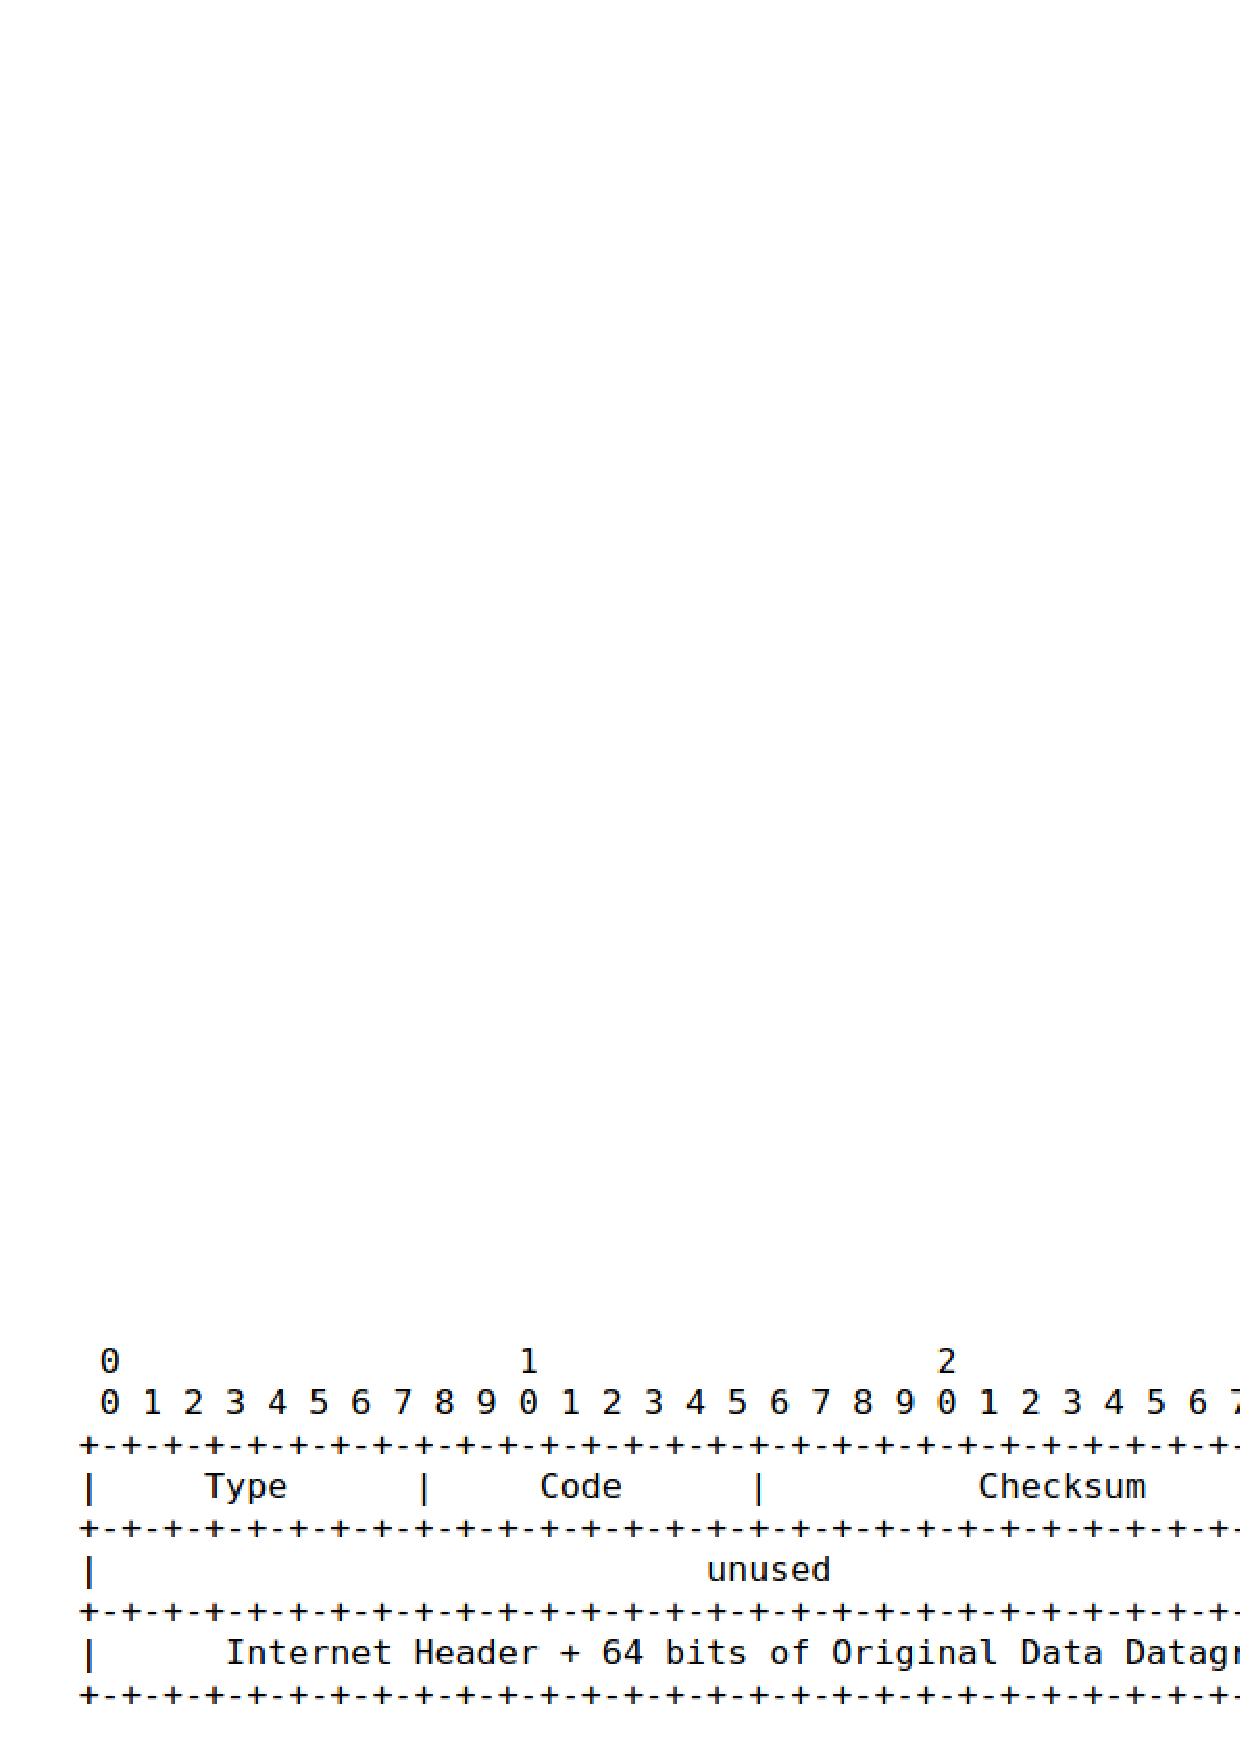
\includegraphics{obr/icmp.png}}
	\caption{ICMP (3, 3)}
	\end{center}
\end{figure}

ICMP s tímto kódem v sobě navíc obsahuje 64 bitů původního datagramu.\cite{icmp}

\newpage

\subsubsection*{ICMPv6}
U ICMPv6 značí nedostupný port typ 1 (\texttt{Destination unreachable}) a kód 4 (\texttt{port unreachable}) \cite{icmp6}.

\begin{figure}[ht]
	\begin{center}
	\scalebox{0.5}{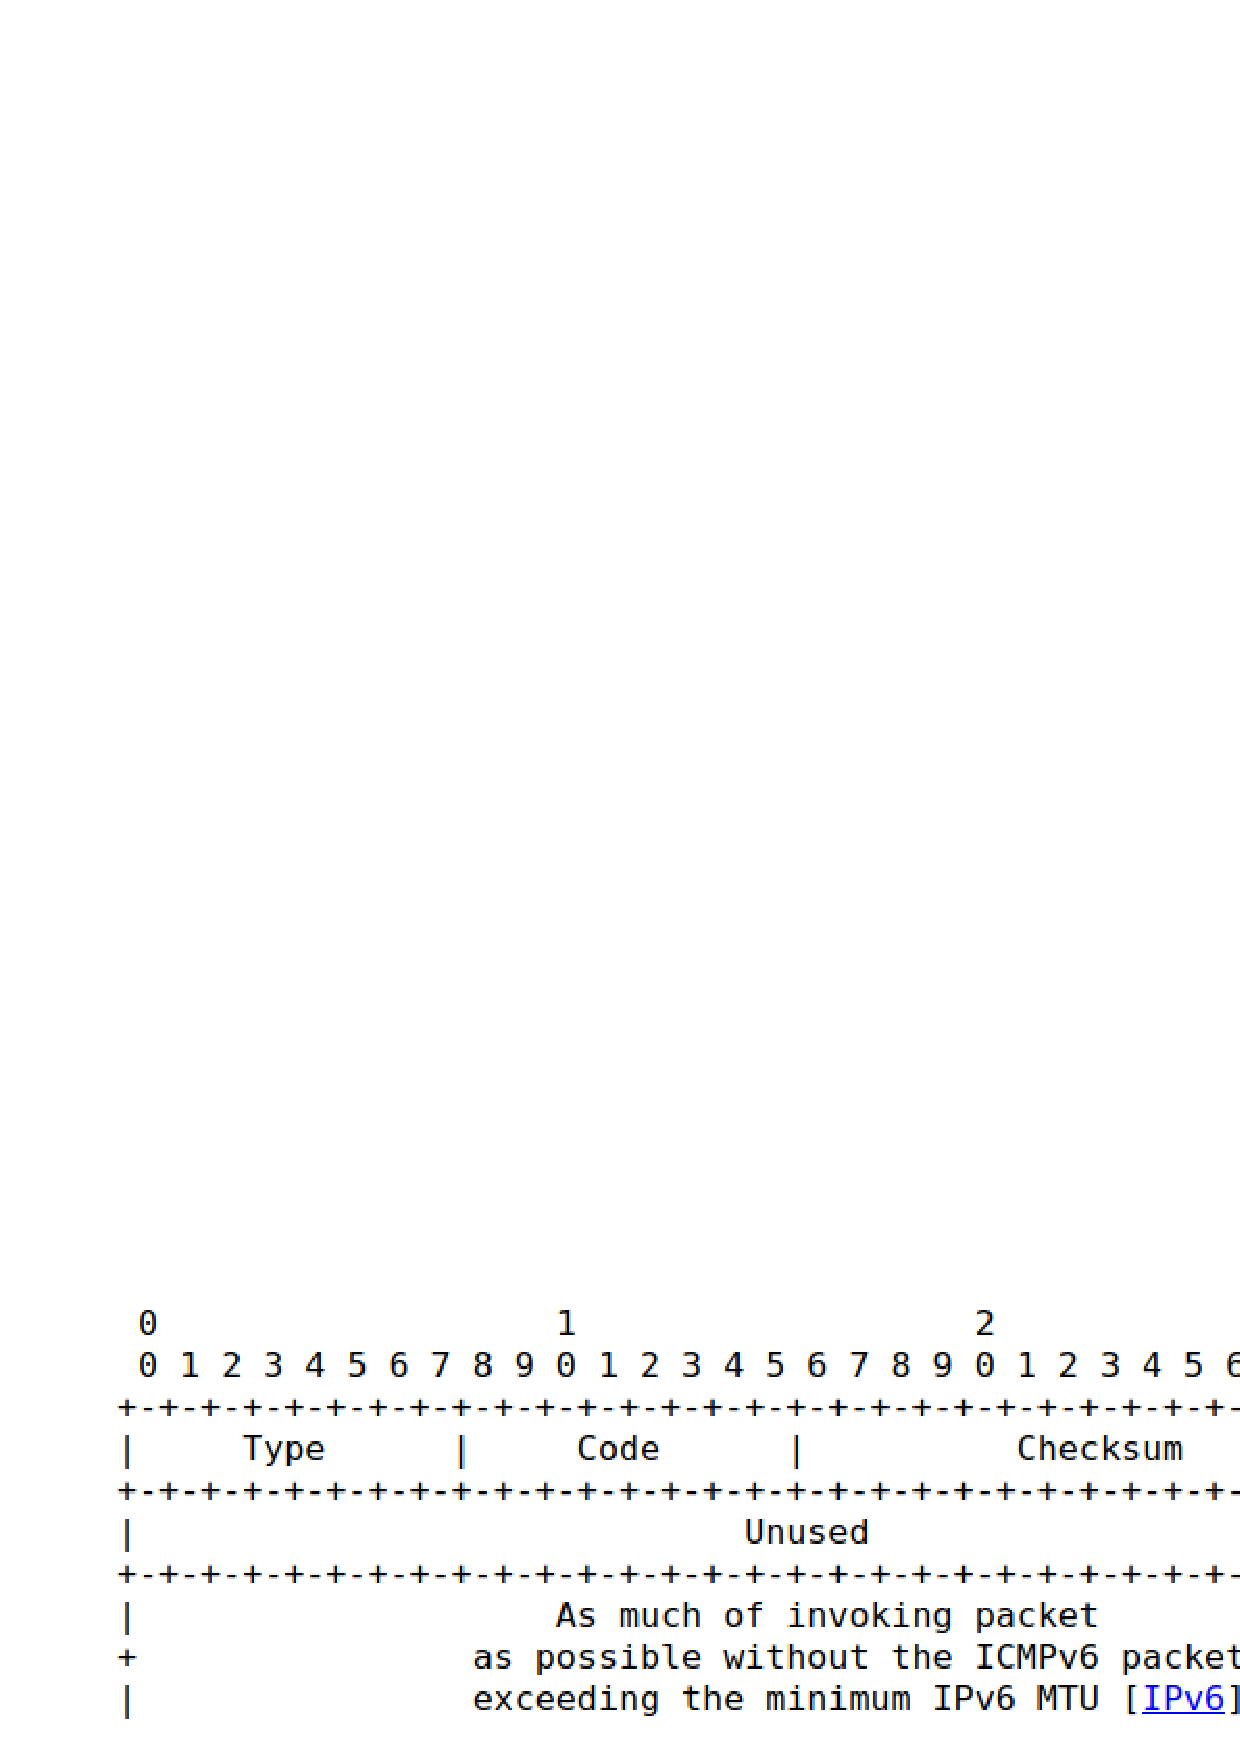
\includegraphics{obr/icmp6.png}}
	\caption{ICMPv6}
	\end{center}
\end{figure}


\subsection{TCP scan}
U TCP protokolu se komunikace navazuje tzv. 3-way-handshakem. Každý typ tohoto hanshaku má nastavené flagy. Při navazování komunikace se odesílá SYN paket. Druhá strana odpovídá SYN-ACK paketem, pokud je port otevřený. Pokud je uzavřený, odpovídá RST paketem. V případě filtrování nepřichází odpověď žádná \cite{wikiScanner}.\\

TCP v sobě nese zdrojový a cílový port, který nás bude zajímat \cite{tcp}. 

\begin{figure}[ht]
	\begin{center}
	\scalebox{0.5}{\includegraphics{obr/tcp.png}}
	\caption{TCP}
	\end{center}
\end{figure}


\section{Implementace}
K implementaci jsem zvolila jazyk \texttt{C++}. \\

Dále jsem využila knihovny \texttt{pcaplib}, \texttt{sys/socket}, \texttt{netinet/in}, \texttt{netinet/udp}, \texttt{arpa/inet}, \texttt{net/ethernet} a \texttt{thread} .

\subsection{UDP scan}
Jak u IPv4, tak IPv6 jsou odesílány pakety na daný port. Pokud přijde daná ICMP zpráva, je označen za uzavřený, jinak za otevřený.\\

Pakety jsou zasílány standartním způsobem pomocí \texttt{sendto}. \\

Jejich odchytávání je realizováno s pomocí knihovny \texttt{pcaplib}. Odchytává se na stejném rozhraní, ze kterého byly pakety poslány, navíc je vždy nastaven filtr pouze na dané ICMP zprávy. Zpracování paketů má na starosti \texttt{pcap\_dispatch} v neblokujícím módu.\\

\subsubsection*{IPv4}
V ICMP samotném není obsažena informace o portu. Tento protokol ale v sobě naštěstí obsahuje kopii dat původního datagramu i s číslem cílového portu. To umožňuje poslat všechny pakety naráz a při odchytávání rozlišovat skenovaný port.\\

Výrazně se tím snižuje doba potřebná k oskenování. Rozdíl mezi časem potřebným k oskenování jedno portu a všech portů je prakticky zanedbatelný.

Abychom se k číslu portu dostali je potřeba znát, kde přesně se v paketu nachází.
Prvních 14 bytů zabírá Ethernet. Pak následuje IP hlavička, ve které se dozvíme celkovou délku IP\cite{packCont} . Za ní je samotné ICMP s tělem obsahující původní IP protokol, a nakonec datagram se zdrojovým a cílovým portem.

\bigskip

\begin{figure}[ht]
	\begin{center}
	\scalebox{0.4}{\includegraphics{obr/icmpWS.png}}
	\caption{Struktura paketu zachyceného WireSharkem}
	\end{center}
\end{figure}

\bigskip

\subsubsection*{IPv6}
U ICMPv6 už ale nelze port nijak vyčíst. Pakety se skenují po jednom, což znamená odeslání paketu, zahájení odchytávání a počkání danou dobu na přijetí. \\

Skenování je proto mnohem pomalejší a závisí na počtu skenovaných portů.\\


\subsection{TCP scan}
Pro nekompletní hanshake je třeba odesílat RAW pakety a dostat se tedy k TCP vrstvě. Toho lze docílit nastavením soketu na typ \texttt{SOCK\_RAW} a protokol \texttt{IPPROTO\_TCP}. U IPv4 se nám tím zpřístupní i IP vrstva.\\

SYN pakety jsou odesílány v jedné vlně.\\

K odchytavání paketů jsem použila opět knihovnu \texttt{pcaplib}. Tentokrát je ale použito dvou   "odchytávačů" se dvěma různými filtry. Jeden pro SYN-ACK pakety (otevřený port), druhý pro RST (uzavřený port).\\

Jak už bylo řečeno, TCP hlavička v sobě obsahuje číslo portu. Stačí se tedy u příchozí zprávy podívat dovnitř paketu, podobně jako u UDP skenování.  Opět to velmi urychluje skenování a není prakticky žádný rozdíl v časové náročnosti scanu jednoho nebo tisíce portů.\\

Pokud k některým portům nepřišla odpověď, je proces zopakován. Bez jakékoliv odpovědi je port označen za filtrovaný.\\

Implementována byla jen verze s IPv4.\\

\section{Testování}
Testování probíhalo na domácí síti a domácím serveru. \\
Ke sledování provozu jsem použila WireShark.


%%%%%%%%%%%%%%%%%%%%%%%%%%%%%%% REF %%%%%%%%%%%%%%%%%%%

\begin{center}
\onecolumn
\renewcommand{\refname}{Zdroje}
\bibliography{cit}
\end{center}
\end{document}

\end{document}
